\documentclass[1p]{elsarticle_modified}
%\bibliographystyle{elsarticle-num}

%\usepackage[colorlinks]{hyperref}
%\usepackage{abbrmath_seonhwa} %\Abb, \Ascr, \Acal ,\Abf, \Afrak
\usepackage{amsfonts}
\usepackage{amssymb}
\usepackage{amsmath}
\usepackage{amsthm}
\usepackage{scalefnt}
\usepackage{amsbsy}
\usepackage{kotex}
\usepackage{caption}
\usepackage{subfig}
\usepackage{color}
\usepackage{graphicx}
\usepackage{xcolor} %% white, black, red, green, blue, cyan, magenta, yellow
\usepackage{float}
\usepackage{setspace}
\usepackage{hyperref}

\usepackage{tikz}
\usetikzlibrary{arrows}

\usepackage{multirow}
\usepackage{array} % fixed length table
\usepackage{hhline}

%%%%%%%%%%%%%%%%%%%%%
\makeatletter
\renewcommand*\env@matrix[1][\arraystretch]{%
	\edef\arraystretch{#1}%
	\hskip -\arraycolsep
	\let\@ifnextchar\new@ifnextchar
	\array{*\c@MaxMatrixCols c}}
\makeatother %https://tex.stackexchange.com/questions/14071/how-can-i-increase-the-line-spacing-in-a-matrix
%%%%%%%%%%%%%%%

\usepackage[normalem]{ulem}

\newcommand{\msout}[1]{\ifmmode\text{\sout{\ensuremath{#1}}}\else\sout{#1}\fi}
%SOURCE: \msout is \stkout macro in https://tex.stackexchange.com/questions/20609/strikeout-in-math-mode

\newcommand{\cancel}[1]{
	\ifmmode
	{\color{red}\msout{#1}}
	\else
	{\color{red}\sout{#1}}
	\fi
}

\newcommand{\add}[1]{
	{\color{blue}\uwave{#1}}
}

\newcommand{\replace}[2]{
	\ifmmode
	{\color{red}\msout{#1}}{\color{blue}\uwave{#2}}
	\else
	{\color{red}\sout{#1}}{\color{blue}\uwave{#2}}
	\fi
}

\newcommand{\Sol}{\mathcal{S}} %segment
\newcommand{\D}{D} %diagram
\newcommand{\A}{\mathcal{A}} %arc


%%%%%%%%%%%%%%%%%%%%%%%%%%%%%5 test

\def\sl{\operatorname{\textup{SL}}(2,\Cbb)}
\def\psl{\operatorname{\textup{PSL}}(2,\Cbb)}
\def\quan{\mkern 1mu \triangleright \mkern 1mu}

\theoremstyle{definition}
\newtheorem{thm}{Theorem}[section]
\newtheorem{prop}[thm]{Proposition}
\newtheorem{lem}[thm]{Lemma}
\newtheorem{ques}[thm]{Question}
\newtheorem{cor}[thm]{Corollary}
\newtheorem{defn}[thm]{Definition}
\newtheorem{exam}[thm]{Example}
\newtheorem{rmk}[thm]{Remark}
\newtheorem{alg}[thm]{Algorithm}

\newcommand{\I}{\sqrt{-1}}
\begin{document}

%\begin{frontmatter}
%
%\title{Boundary parabolic representations of knots up to 8 crossings}
%
%%% Group authors per affiliation:
%\author{Yunhi Cho} 
%\address{Department of Mathematics, University of Seoul, Seoul, Korea}
%\ead{yhcho@uos.ac.kr}
%
%
%\author{Seonhwa Kim} %\fnref{s_kim}}
%\address{Center for Geometry and Physics, Institute for Basic Science, Pohang, 37673, Korea}
%\ead{ryeona17@ibs.re.kr}
%
%\author{Hyuk Kim}
%\address{Department of Mathematical Sciences, Seoul National University, Seoul 08826, Korea}
%\ead{hyukkim@snu.ac.kr}
%
%\author{Seokbeom Yoon}
%\address{Department of Mathematical Sciences, Seoul National University, Seoul, 08826,  Korea}
%\ead{sbyoon15@snu.ac.kr}
%
%\begin{abstract}
%We find all boundary parabolic representation of knots up to 8 crossings.
%
%\end{abstract}
%\begin{keyword}
%    \MSC[2010] 57M25 
%\end{keyword}
%
%\end{frontmatter}

%\linenumbers
%\tableofcontents
%
\newcommand\colored[1]{\textcolor{white}{\rule[-0.35ex]{0.8em}{1.4ex}}\kern-0.8em\color{red} #1}%
%\newcommand\colored[1]{\textcolor{white}{ #1}\kern-2.17ex	\textcolor{white}{ #1}\kern-1.81ex	\textcolor{white}{ #1}\kern-2.15ex\color{red}#1	}

{\Large $\underline{11a_{204}~(K11a_{204})}$}

\setlength{\tabcolsep}{10pt}
\renewcommand{\arraystretch}{1.6}
\vspace{1cm}\begin{tabular}{m{100pt}>{\centering\arraybackslash}m{274pt}}
\multirow{5}{120pt}{
	\centering
	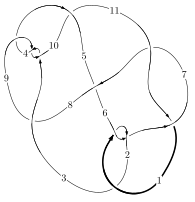
\includegraphics[width=112pt]{../../../GIT/diagram.site/Diagrams/png/453_11a_204.png}\\
\ \ \ A knot diagram\footnotemark}&
\allowdisplaybreaks
\textbf{Linearized knot diagam} \\
\cline{2-2}
 &
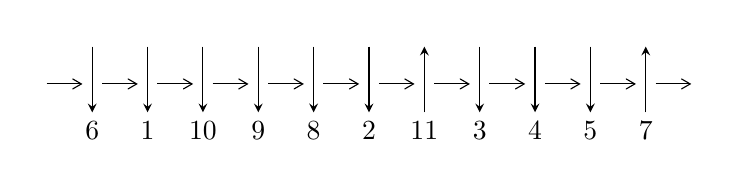
\begin{tikzpicture}[x=20pt, y=17pt]
	% nodes
	\node (C0) at (0, 0) {};
	\node (C1) at (1, 0) {};
	\node (C1U) at (1, +1) {};
	\node (C1D) at (1, -1) {6};

	\node (C2) at (2, 0) {};
	\node (C2U) at (2, +1) {};
	\node (C2D) at (2, -1) {1};

	\node (C3) at (3, 0) {};
	\node (C3U) at (3, +1) {};
	\node (C3D) at (3, -1) {10};

	\node (C4) at (4, 0) {};
	\node (C4U) at (4, +1) {};
	\node (C4D) at (4, -1) {9};

	\node (C5) at (5, 0) {};
	\node (C5U) at (5, +1) {};
	\node (C5D) at (5, -1) {8};

	\node (C6) at (6, 0) {};
	\node (C6U) at (6, +1) {};
	\node (C6D) at (6, -1) {2};

	\node (C7) at (7, 0) {};
	\node (C7U) at (7, +1) {};
	\node (C7D) at (7, -1) {11};

	\node (C8) at (8, 0) {};
	\node (C8U) at (8, +1) {};
	\node (C8D) at (8, -1) {3};

	\node (C9) at (9, 0) {};
	\node (C9U) at (9, +1) {};
	\node (C9D) at (9, -1) {4};

	\node (C10) at (10, 0) {};
	\node (C10U) at (10, +1) {};
	\node (C10D) at (10, -1) {5};

	\node (C11) at (11, 0) {};
	\node (C11U) at (11, +1) {};
	\node (C11D) at (11, -1) {7};
	\node (C12) at (12, 0) {};

	% arrows
	\draw[->,>={angle 60}]
	(C0) edge (C1) (C1) edge (C2) (C2) edge (C3) (C3) edge (C4) (C4) edge (C5) (C5) edge (C6) (C6) edge (C7) (C7) edge (C8) (C8) edge (C9) (C9) edge (C10) (C10) edge (C11) (C11) edge (C12) ;	\draw[->,>=stealth]
	(C1U) edge (C1D) (C2U) edge (C2D) (C3U) edge (C3D) (C4U) edge (C4D) (C5U) edge (C5D) (C6U) edge (C6D) (C7D) edge (C7U) (C8U) edge (C8D) (C9U) edge (C9D) (C10U) edge (C10D) (C11D) edge (C11U) ;
	\end{tikzpicture} \\
\hhline{~~} \\& 
\textbf{Solving Sequence} \\ \cline{2-2} 
 &
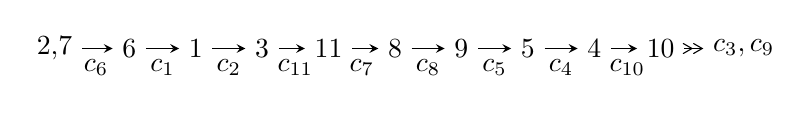
\begin{tikzpicture}[x=24pt, y=7pt]
	% node
	\node (A0) at (-1/8, 0) {2,7};
	\node (A1) at (1, 0) {6};
	\node (A2) at (2, 0) {1};
	\node (A3) at (3, 0) {3};
	\node (A4) at (4, 0) {11};
	\node (A5) at (5, 0) {8};
	\node (A6) at (6, 0) {9};
	\node (A7) at (7, 0) {5};
	\node (A8) at (8, 0) {4};
	\node (A9) at (9, 0) {10};
	\node (C1) at (1/2, -1) {$c_{6}$};
	\node (C2) at (3/2, -1) {$c_{1}$};
	\node (C3) at (5/2, -1) {$c_{2}$};
	\node (C4) at (7/2, -1) {$c_{11}$};
	\node (C5) at (9/2, -1) {$c_{7}$};
	\node (C6) at (11/2, -1) {$c_{8}$};
	\node (C7) at (13/2, -1) {$c_{5}$};
	\node (C8) at (15/2, -1) {$c_{4}$};
	\node (C9) at (17/2, -1) {$c_{10}$};
	\node (A10) at (41/4, 0) {$c_{3},c_{9}$};

	% edge
	\draw[->,>=stealth]	
	(A0) edge (A1) (A1) edge (A2) (A2) edge (A3) (A3) edge (A4) (A4) edge (A5) (A5) edge (A6) (A6) edge (A7) (A7) edge (A8) (A8) edge (A9) ;
	\draw[->>,>={angle 60}]	
	(A9) edge (A10);
\end{tikzpicture} \\ 

\end{tabular} \\

\footnotetext{
The image of knot diagram is generated by the software ``\textbf{Draw programme}" developed by Andrew Bartholomew(\url{http://www.layer8.co.uk/maths/draw/index.htm\#Running-draw}), where we modified some parts for our purpose(\url{https://github.com/CATsTAILs/LinksPainter}).
}\phantom \\ \newline 
\centering \textbf{Ideals for irreducible components\footnotemark of $X_{\text{par}}$} 
 
\begin{align*}
I^u_{1}&=\langle 
u^{50}- u^{49}+\cdots+u-1\rangle \\
\\
\end{align*}
\raggedright * 1 irreducible components of $\dim_{\mathbb{C}}=0$, with total 50 representations.\\
\footnotetext{All coefficients of polynomials are rational numbers. But the coefficients are sometimes approximated in decimal forms when there is not enough margin.}
\newpage
\renewcommand{\arraystretch}{1}
\centering \section*{I. $I^u_{1}= \langle u^{50}- u^{49}+\cdots+u-1 \rangle$}
\flushleft \textbf{(i) Arc colorings}\\
\begin{tabular}{m{7pt} m{180pt} m{7pt} m{180pt} }
\flushright $a_{2}=$&$\begin{pmatrix}0\\u\end{pmatrix}$ \\
\flushright $a_{7}=$&$\begin{pmatrix}1\\0\end{pmatrix}$ \\
\flushright $a_{6}=$&$\begin{pmatrix}1\\- u^2\end{pmatrix}$ \\
\flushright $a_{1}=$&$\begin{pmatrix}u\\- u^3+u\end{pmatrix}$ \\
\flushright $a_{3}=$&$\begin{pmatrix}- u^3\\u^5- u^3+u\end{pmatrix}$ \\
\flushright $a_{11}=$&$\begin{pmatrix}u^3\\- u^3+u\end{pmatrix}$ \\
\flushright $a_{8}=$&$\begin{pmatrix}u^6- u^4+1\\- u^6+2 u^4- u^2\end{pmatrix}$ \\
\flushright $a_{9}=$&$\begin{pmatrix}- u^{14}+3 u^{12}-4 u^{10}+u^8+2 u^6-2 u^4+1\\u^{16}-4 u^{14}+8 u^{12}-8 u^{10}+4 u^8\end{pmatrix}$ \\
\flushright $a_{5}=$&$\begin{pmatrix}- u^{14}+3 u^{12}-4 u^{10}+u^8+2 u^6-2 u^4+1\\u^{14}-4 u^{12}+7 u^{10}-6 u^8+2 u^6- u^2\end{pmatrix}$ \\
\flushright $a_{4}=$&$\begin{pmatrix}- u^{44}+11 u^{42}+\cdots- u^2+1\\u^{46}-12 u^{44}+\cdots+2 u^6- u^2\end{pmatrix}$ \\
\flushright $a_{10}=$&$\begin{pmatrix}- u^{25}+6 u^{23}+\cdots-3 u^5+u\\u^{25}-7 u^{23}+\cdots-2 u^3+u\end{pmatrix}$\\ \flushright $a_{10}=$&$\begin{pmatrix}- u^{25}+6 u^{23}+\cdots-3 u^5+u\\u^{25}-7 u^{23}+\cdots-2 u^3+u\end{pmatrix}$\\&\end{tabular}
\flushleft \textbf{(ii) Obstruction class $= -1$}\\~\\
\flushleft \textbf{(iii) Cusp Shapes $= -4 u^{48}+52 u^{46}+\cdots+8 u-6$}\\~\\
\newpage\renewcommand{\arraystretch}{1}
\flushleft \textbf{(iv) u-Polynomials at the component}\newline \\
\begin{tabular}{m{50pt}|m{274pt}}
Crossings & \hspace{64pt}u-Polynomials at each crossing \\
\hline $$\begin{aligned}c_{1},c_{6}\end{aligned}$$&$\begin{aligned}
&u^{50}- u^{49}+\cdots+u-1
\end{aligned}$\\
\hline $$\begin{aligned}c_{2}\end{aligned}$$&$\begin{aligned}
&u^{50}+27 u^{49}+\cdots+3 u+1
\end{aligned}$\\
\hline $$\begin{aligned}c_{3},c_{4},c_{9}\end{aligned}$$&$\begin{aligned}
&u^{50}+u^{49}+\cdots-3 u-1
\end{aligned}$\\
\hline $$\begin{aligned}c_{5}\end{aligned}$$&$\begin{aligned}
&u^{50}-7 u^{49}+\cdots-111 u+37
\end{aligned}$\\
\hline $$\begin{aligned}c_{7},c_{11}\end{aligned}$$&$\begin{aligned}
&u^{50}-3 u^{49}+\cdots+u+1
\end{aligned}$\\
\hline $$\begin{aligned}c_{8},c_{10}\end{aligned}$$&$\begin{aligned}
&u^{50}- u^{49}+\cdots-45 u-17
\end{aligned}$\\
\hline
\end{tabular}\\~\\
\newpage\renewcommand{\arraystretch}{1}
\flushleft \textbf{(v) Riley Polynomials at the component}\newline \\
\begin{tabular}{m{50pt}|m{274pt}}
Crossings & \hspace{64pt}Riley Polynomials at each crossing \\
\hline $$\begin{aligned}c_{1},c_{6}\end{aligned}$$&$\begin{aligned}
&y^{50}-27 y^{49}+\cdots-3 y+1
\end{aligned}$\\
\hline $$\begin{aligned}c_{2}\end{aligned}$$&$\begin{aligned}
&y^{50}-7 y^{49}+\cdots-7 y+1
\end{aligned}$\\
\hline $$\begin{aligned}c_{3},c_{4},c_{9}\end{aligned}$$&$\begin{aligned}
&y^{50}+41 y^{49}+\cdots-3 y+1
\end{aligned}$\\
\hline $$\begin{aligned}c_{5}\end{aligned}$$&$\begin{aligned}
&y^{50}-11 y^{49}+\cdots-28823 y+1369
\end{aligned}$\\
\hline $$\begin{aligned}c_{7},c_{11}\end{aligned}$$&$\begin{aligned}
&y^{50}+41 y^{49}+\cdots-111 y+1
\end{aligned}$\\
\hline $$\begin{aligned}c_{8},c_{10}\end{aligned}$$&$\begin{aligned}
&y^{50}-35 y^{49}+\cdots+457 y+289
\end{aligned}$\\
\hline
\end{tabular}\\~\\
\newpage\flushleft \textbf{(vi) Complex Volumes and Cusp Shapes}
$$\begin{array}{c|c|c}  
\text{Solutions to }I^u_{1}& \I (\text{vol} + \sqrt{-1}CS) & \text{Cusp shape}\\
 \hline 
\begin{aligned}
u &= -0.898377 + 0.505512 I\end{aligned}
 & -2.14014 + 4.60582 I & -9.82761 - 7.01636 I \\ \hline\begin{aligned}
u &= -0.898377 - 0.505512 I\end{aligned}
 & -2.14014 - 4.60582 I & -9.82761 + 7.01636 I \\ \hline\begin{aligned}
u &= \phantom{-}0.886274 + 0.537129 I\end{aligned}
 & \phantom{-}2.36766 - 8.44259 I & -4.56565 + 8.69974 I \\ \hline\begin{aligned}
u &= \phantom{-}0.886274 - 0.537129 I\end{aligned}
 & \phantom{-}2.36766 + 8.44259 I & -4.56565 - 8.69974 I \\ \hline\begin{aligned}
u &= \phantom{-}0.940835 + 0.435517 I\end{aligned}
 & \phantom{-}1.03261 - 1.03580 I & -6.91855 + 2.91618 I \\ \hline\begin{aligned}
u &= \phantom{-}0.940835 - 0.435517 I\end{aligned}
 & \phantom{-}1.03261 + 1.03580 I & -6.91855 - 2.91618 I \\ \hline\begin{aligned}
u &= \phantom{-}1.04249\phantom{ +0.000000I}\end{aligned}
 & -5.57110\phantom{ +0.000000I} & -16.4420\phantom{ +0.000000I} \\ \hline\begin{aligned}
u &= -1.048370 + 0.049358 I\end{aligned}
 & -1.64759 + 4.00369 I & -11.91063 - 3.67666 I \\ \hline\begin{aligned}
u &= -1.048370 - 0.049358 I\end{aligned}
 & -1.64759 - 4.00369 I & -11.91063 + 3.67666 I \\ \hline\begin{aligned}
u &= -0.764066 + 0.531630 I\end{aligned}
 & \phantom{-}6.63211 + 2.15686 I & \phantom{-}0.57370 - 3.89945 I \\ \hline\begin{aligned}
u &= -0.764066 - 0.531630 I\end{aligned}
 & \phantom{-}6.63211 - 2.15686 I & \phantom{-}0.57370 + 3.89945 I \\ \hline\begin{aligned}
u &= \phantom{-}0.774496 + 0.423862 I\end{aligned}
 & \phantom{-}0.95587 - 1.83688 I & -2.97268 + 5.52059 I \\ \hline\begin{aligned}
u &= \phantom{-}0.774496 - 0.423862 I\end{aligned}
 & \phantom{-}0.95587 + 1.83688 I & -2.97268 - 5.52059 I \\ \hline\begin{aligned}
u &= \phantom{-}0.131214 + 0.816301 I\end{aligned}
 & -1.25862 + 8.74450 I & -6.26482 - 5.70892 I \\ \hline\begin{aligned}
u &= \phantom{-}0.131214 - 0.816301 I\end{aligned}
 & -1.25862 - 8.74450 I & -6.26482 + 5.70892 I \\ \hline\begin{aligned}
u &= -0.113334 + 0.813002 I\end{aligned}
 & -5.75677 - 4.53837 I & -10.90083 + 3.52404 I \\ \hline\begin{aligned}
u &= -0.113334 - 0.813002 I\end{aligned}
 & -5.75677 + 4.53837 I & -10.90083 - 3.52404 I \\ \hline\begin{aligned}
u &= \phantom{-}0.600001 + 0.552718 I\end{aligned}
 & \phantom{-}3.16690 + 4.05720 I & -2.39559 - 2.41761 I \\ \hline\begin{aligned}
u &= \phantom{-}0.600001 - 0.552718 I\end{aligned}
 & \phantom{-}3.16690 - 4.05720 I & -2.39559 + 2.41761 I \\ \hline\begin{aligned}
u &= \phantom{-}0.088090 + 0.807114 I\end{aligned}
 & -2.52256 + 0.29931 I & -7.87191 + 0.33424 I \\ \hline\begin{aligned}
u &= \phantom{-}0.088090 - 0.807114 I\end{aligned}
 & -2.52256 - 0.29931 I & -7.87191 - 0.33424 I \\ \hline\begin{aligned}
u &= \phantom{-}1.124710 + 0.394492 I\end{aligned}
 & \phantom{-}0.834215 - 0.681511 I & -6.55623 + 0. I\phantom{ +0.000000I} \\ \hline\begin{aligned}
u &= \phantom{-}1.124710 - 0.394492 I\end{aligned}
 & \phantom{-}0.834215 + 0.681511 I & -6.55623 + 0. I\phantom{ +0.000000I} \\ \hline\begin{aligned}
u &= -1.169100 + 0.434672 I\end{aligned}
 & -4.41097 + 2.59787 I & -11.45875 + 0. I\phantom{ +0.000000I} \\ \hline\begin{aligned}
u &= -1.169100 - 0.434672 I\end{aligned}
 & -4.41097 - 2.59787 I & -11.45875 + 0. I\phantom{ +0.000000I} \\ \hline\begin{aligned}
u &= -1.157340 + 0.497610 I\end{aligned}
 & \phantom{-}1.58916 + 7.35454 I & \phantom{-0.000000 } 0 \\ \hline\begin{aligned}
u &= -1.157340 - 0.497610 I\end{aligned}
 & \phantom{-}1.58916 - 7.35454 I & \phantom{-0.000000 } 0 \\ \hline\begin{aligned}
u &= -0.542490 + 0.497935 I\end{aligned}
 & -1.186550 - 0.458750 I & -7.63805 + 0.36311 I \\ \hline\begin{aligned}
u &= -0.542490 - 0.497935 I\end{aligned}
 & -1.186550 + 0.458750 I & -7.63805 - 0.36311 I \\ \hline\begin{aligned}
u &= \phantom{-}1.173630 + 0.470826 I\end{aligned}
 & -4.14754 - 5.79334 I & \phantom{-0.000000 } 0\\
 \hline 
 \end{array}$$\newpage$$\begin{array}{c|c|c}  
\text{Solutions to }I^u_{1}& \I (\text{vol} + \sqrt{-1}CS) & \text{Cusp shape}\\
 \hline 
\begin{aligned}
u &= \phantom{-}1.173630 - 0.470826 I\end{aligned}
 & -4.14754 + 5.79334 I & \phantom{-0.000000 } 0 \\ \hline\begin{aligned}
u &= -0.173744 + 0.706786 I\end{aligned}
 & \phantom{-}4.42834 - 2.79951 I & -1.47445 + 3.26453 I \\ \hline\begin{aligned}
u &= -0.173744 - 0.706786 I\end{aligned}
 & \phantom{-}4.42834 + 2.79951 I & -1.47445 - 3.26453 I \\ \hline\begin{aligned}
u &= -1.219870 + 0.382444 I\end{aligned}
 & -5.33475 - 4.67917 I & \phantom{-0.000000 } 0 \\ \hline\begin{aligned}
u &= -1.219870 - 0.382444 I\end{aligned}
 & -5.33475 + 4.67917 I & \phantom{-0.000000 } 0 \\ \hline\begin{aligned}
u &= \phantom{-}1.219490 + 0.394041 I\end{aligned}
 & -9.75574 + 0.40809 I & \phantom{-0.000000 } 0 \\ \hline\begin{aligned}
u &= \phantom{-}1.219490 - 0.394041 I\end{aligned}
 & -9.75574 - 0.40809 I & \phantom{-0.000000 } 0 \\ \hline\begin{aligned}
u &= -1.217770 + 0.408433 I\end{aligned}
 & -6.41473 + 3.90979 I & \phantom{-0.000000 } 0 \\ \hline\begin{aligned}
u &= -1.217770 - 0.408433 I\end{aligned}
 & -6.41473 - 3.90979 I & \phantom{-0.000000 } 0 \\ \hline\begin{aligned}
u &= \phantom{-}0.065064 + 0.701160 I\end{aligned}
 & -1.00563 + 1.42365 I & -7.09664 - 4.59801 I \\ \hline\begin{aligned}
u &= \phantom{-}0.065064 - 0.701160 I\end{aligned}
 & -1.00563 - 1.42365 I & -7.09664 + 4.59801 I \\ \hline\begin{aligned}
u &= \phantom{-}1.203910 + 0.493230 I\end{aligned}
 & -5.81092 - 5.03608 I & \phantom{-0.000000 } 0 \\ \hline\begin{aligned}
u &= \phantom{-}1.203910 - 0.493230 I\end{aligned}
 & -5.81092 + 5.03608 I & \phantom{-0.000000 } 0 \\ \hline\begin{aligned}
u &= -1.202290 + 0.504191 I\end{aligned}
 & -8.97338 + 9.35305 I & \phantom{-0.000000 } 0 \\ \hline\begin{aligned}
u &= -1.202290 - 0.504191 I\end{aligned}
 & -8.97338 - 9.35305 I & \phantom{-0.000000 } 0 \\ \hline\begin{aligned}
u &= \phantom{-}1.200010 + 0.511632 I\end{aligned}
 & -4.4198 - 13.6080 I & \phantom{-0.000000 } 0 \\ \hline\begin{aligned}
u &= \phantom{-}1.200010 - 0.511632 I\end{aligned}
 & -4.4198 + 13.6080 I & \phantom{-0.000000 } 0 \\ \hline\begin{aligned}
u &= \phantom{-}0.406824 + 0.539325 I\end{aligned}
 & \phantom{-}2.56296 - 2.88378 I & -2.70702 + 3.08785 I \\ \hline\begin{aligned}
u &= \phantom{-}0.406824 - 0.539325 I\end{aligned}
 & \phantom{-}2.56296 + 2.88378 I & -2.70702 - 3.08785 I \\ \hline\begin{aligned}
u &= -0.658085\phantom{ +0.000000I}\end{aligned}
 & -0.823669\phantom{ +0.000000I} & -13.0660\phantom{ +0.000000I}\\
 \hline 
 \end{array}$$\newpage
\newpage\renewcommand{\arraystretch}{1}
\centering \section*{ II. u-Polynomials}
\begin{tabular}{m{50pt}|m{274pt}}
Crossings & \hspace{64pt}u-Polynomials at each crossing \\
\hline $$\begin{aligned}c_{1},c_{6}\end{aligned}$$&$\begin{aligned}
&u^{50}- u^{49}+\cdots+u-1
\end{aligned}$\\
\hline $$\begin{aligned}c_{2}\end{aligned}$$&$\begin{aligned}
&u^{50}+27 u^{49}+\cdots+3 u+1
\end{aligned}$\\
\hline $$\begin{aligned}c_{3},c_{4},c_{9}\end{aligned}$$&$\begin{aligned}
&u^{50}+u^{49}+\cdots-3 u-1
\end{aligned}$\\
\hline $$\begin{aligned}c_{5}\end{aligned}$$&$\begin{aligned}
&u^{50}-7 u^{49}+\cdots-111 u+37
\end{aligned}$\\
\hline $$\begin{aligned}c_{7},c_{11}\end{aligned}$$&$\begin{aligned}
&u^{50}-3 u^{49}+\cdots+u+1
\end{aligned}$\\
\hline $$\begin{aligned}c_{8},c_{10}\end{aligned}$$&$\begin{aligned}
&u^{50}- u^{49}+\cdots-45 u-17
\end{aligned}$\\
\hline
\end{tabular}\newpage\renewcommand{\arraystretch}{1}
\centering \section*{ III. Riley Polynomials}
\begin{tabular}{m{50pt}|m{274pt}}
Crossings & \hspace{64pt}Riley Polynomials at each crossing \\
\hline $$\begin{aligned}c_{1},c_{6}\end{aligned}$$&$\begin{aligned}
&y^{50}-27 y^{49}+\cdots-3 y+1
\end{aligned}$\\
\hline $$\begin{aligned}c_{2}\end{aligned}$$&$\begin{aligned}
&y^{50}-7 y^{49}+\cdots-7 y+1
\end{aligned}$\\
\hline $$\begin{aligned}c_{3},c_{4},c_{9}\end{aligned}$$&$\begin{aligned}
&y^{50}+41 y^{49}+\cdots-3 y+1
\end{aligned}$\\
\hline $$\begin{aligned}c_{5}\end{aligned}$$&$\begin{aligned}
&y^{50}-11 y^{49}+\cdots-28823 y+1369
\end{aligned}$\\
\hline $$\begin{aligned}c_{7},c_{11}\end{aligned}$$&$\begin{aligned}
&y^{50}+41 y^{49}+\cdots-111 y+1
\end{aligned}$\\
\hline $$\begin{aligned}c_{8},c_{10}\end{aligned}$$&$\begin{aligned}
&y^{50}-35 y^{49}+\cdots+457 y+289
\end{aligned}$\\
\hline
\end{tabular}
\vskip 2pc
\end{document}